% ---------------------------------------------------------------------------
% Author guideline and sample document for EG publication using LaTeX2e input
% D.Fellner, v1.12, Nov 01, 2006

\documentclass{egpubl}
\usepackage{sbim09}

% --- for  Annual CONFERENCE
% \ConferenceSubmission % uncomment for Conference submission
% \ConferencePaper      % uncomment for (final) Conference Paper
% \STAR                 % uncomment for STAR contribution
% \Tutorial             % uncomment for Tutorial contribution
% \ShortPresentation    % uncomment for (final) Short Conference Presentation
%
% --- for  CGF Journal
% \JournalSubmission    % uncomment for submission to Computer Graphics Forum
% \JournalPaper         % uncomment for final version of Journal Paper
%
% --- for  EG Workshop Proceedings
\WsSubmission    % uncomment for submission to EG Workshop
% \WsPaper         % uncomment for final version of EG Workshop contribution
%
 \electronicVersion % can be used both for the printed and electronic version

% !! *please* don't change anything above
% !! unless you REALLY know what you are doing
% ------------------------------------------------------------------------

% for including postscript figures
% mind: package option 'draft' will replace PS figure by a filename within a frame
\ifpdf \usepackage[pdftex]{graphicx} \pdfcompresslevel=9
\else \usepackage[dvips]{graphicx} \fi

\PrintedOrElectronic

% prepare for electronic version of your document
\usepackage{t1enc,dfadobe}

\usepackage{egweblnk}
\usepackage{cite}

% For backwards compatibility to old LaTeX type font selection.
% Uncomment if your document adheres to LaTeX2e recommendations.
\let\rm=\rmfamily    \let\sf=\sffamily    \let\tt=\ttfamily
\let\it=\itshape     \let\sl=\slshape     \let\sc=\scshape
\let\bf=\bfseries

% end of prologue

\title[The Effect of Task on Classification Accuracy]%
      {The Effect of Task on Classification Accuracy: Using Gesture Recognition Techniques 
      in Free-Sketch Recognition}

% for anonymous conference submission please enter your SUBMISSION ID
% instead of the author's name (and leave the affiliation blank) !!
\author[1010]
       {1010%$^{1,2}$
        %\\
         %$^1$Harvey Mudd College\\
         %$^2$University of California, Riverside
       }

% ------------------------------------------------------------------------

% if the Editors-in-Chief have given you the data, you may uncomment
% the following five lines and insert it here
%
% \volume{27}   % the volume in which the issue will be published;
% \issue{1}     % the issue number of the publication
% \pStartPage{1}      % set starting page


%-------------------------------------------------------------------------
\begin{document}

\maketitle

\begin{abstract}
Generating, grouping, and labeling free-sketch data is a difficult and time-consuming task for both user study participants and researchers. To simplify this process for both parties, we would like to have users draw isolated shapes instead of complete sketches that must be hand-labeled and grouped, and then use this data to train our free-sketch symbol recognizer.  However, it is an open question whether shapes draw in isolation accurately reflect the way users draw shapes in a complete diagram.  Furthermore, many of the simplest shape recognition algorithms were designed to recognizer gestures, and it is not clear that they will generalize to freely-draw shapes.  To answer these questions, we perform experiments using three different recognizers to measure the effect of data collection task on recognition accuracy.  We find that recognizers trained only on isolated shapes can classify free-sketched shapes as well as the same recognizer trained on free-sketches. We also show that user-specific training examples significantly improve recognition rates.  Finally, we introduce a variant of a popular and simple gesture recognition algorithm that recognizes freely-drawn shapes as well as a highly-accurate but more complex recognizer designed explicitly for free-sketch recognition.  

\begin{classification} % according to http://www.acm.org/class/1998/
\CCScat{Information interfaces and presentation}{H.5.2}{User Interfaces}{Interaction styles}
\CCScat{Pattern recognition}{I.5.2}{Design methodology}{Classifier design and evaluation}
\CCScat{Pattern recognition}{I.5.5}{Implementation}{Interactive systems}
\end{classification}

\end{abstract}


%-------------------------------------------------------------------------
\section{Introduction}
Having realistic training data is essential to developing robust
recognition algorithms.  Obtaining such data for sketch recognition 
can be an arduous process. Public data sets are
emerging~\cite{Oltmans2004ETCHASketch,Hse2005Recognition,
  Wolin2007Labeler,Paulson2008SOUSA,Blagojevic2008Data}, but these
necessarily represent a limited number of domains and often include
only shapes drawn in isolation, rather than complete sketches.

Many of the most robust and complete sketch recognition systems today
(e.g., \cite{Zeleznik2008Lineogrammer} and~\cite{Lee2008Newton}) focus
on gesture or isolated symbol recognition rather than the more
difficult problem of free-sketch recognition.  Such systems constrain
users to draw shapes one at a time, avoiding the considerable
difficulties of finding the boundaries between them.  Gesture
recognition additionally constrains the user to drawing each shape
with a specific style (e.g., users might be required to draw
rectangles with a single clockwise pen stroke), minimizing drawing
style variation.

Because of these simplifications, collecting training data for gesture
recognizers is (relatively) straightforward.  Users can be prompted to
draw each gesture individually, without need for any manual processing
or labeling.  Because of the limited variation in drawing style, a
recognizer trained on data from one set of users is likely to work
well for other users. Additionally, many gesture recognition
algorithms (e.g.~\cite{dollar}) can be fine-tuned for an individual
user by simply having them draw a few examples.

Obtaining training-data for free-sketch recognition systems is
considerably more difficult than for gesture-based systems. In recent
years, researchers have developed several tools to facilitate the
collection and labeling of data
\cite{Wolin2007Labeler,Paulson2008SOUSA,Blagojevic2008Data}.  However,
even with these tools, processing the data is still a labor and
time-intensive task because the pen strokes must be manually grouped
into individual symbols and labeled.  Furthermore, most of these tools
are designed for researchers. It would be impractical for an end-user
to manually group and label the symbols in a free-sketch to improve a
system's recognition performance.


For these reasons, researchers frequently obtain recognition training
data for free-sketch recognition systems using the same simplified
data collection process suitable for gesture-based systems (e.g.,
\cite{Kara2005ImageBased,Hse2004ssr}). In the current work, we seek to
evaluate the soundness of this approach, explicitly examining the useful
of symbols drawn in isolation for training shape recognizers for
free-sketch recognition.  The answer to this question is not obvious
as drawing isolated symbols is not the same as drawing them in the
context of a larger task. For instance, drawing a logic gate by itself
is substantially different from designing a digital circuit.  In the
former case, the user's focus is on the drawing task, while in the
latter, the user's focus is likely to be the \textit{design} task.

To answer this question, we conducted a study in which participants
were asked to perform sketching tasks of varying
complexity. Specifically, participants were asked to draw logic gates
in isolation, copy digital circuits, and synthesize and sketch new
circuit designs.  We then examine how recognition accuracy varied
with the task used to obtain training data.

The other piece of this work is to explore how well simple gesture recognition 
algorithms can be applied to more complex recognition problems.  
We address the question: can existing gesture recognition algorithms easily 
be modified to perform well on shapes drawn freely? 

We show that recognition accuracy is not highly dependent on the task
users performed when generating training data.  Simple isolated symbol
data works just as well for training symbol recognizers as symbols
extracted from complex sketches. We also show that including
user-specific examples in the training process gives a significant
boost to accuracy, but that we can produce highly accurate recognizers
even without user-specific examples.  Second, we present a variant of
the recently proposed and very popular \$1 recognizer~\cite{dollar}
that works on freely-drawn shapes comprised of any number of strokes
drawn in any order.  While necessarily more complicated than the
original, our variant maintains much of the simplicity of the original
algorithm, can be implemented quickly and easily, and performs with
comparable accuracy to a more complex algorithm designed specifically
for recognizing freely-drawn shapes.

%-------------------------------------------------------------------------
\section{Background}
The central focus of this paper is to determine whether potential drawing style variations impact symbol recognition accuracy from one task to another.  Relatively few studies have examined how people draw, and no study that we are aware of has compared drawing styles across tasks.  Oltmans et al. present some preliminary observations from sketches from multiple domains~\cite{Oltmans2004ETCHASketch}.  Although collected in a laboratory, these sketches simulate natural drawing style as users were asked to produce an original design rather than copy an existing diagram or draw specific shapes.  Alvarado and Lazzareschi analyze drawings made by students in an circuit design class as part of their routine work for the class~\cite{Alvarado2007Properties}.  They find that drawing styles vary across users and even across the sketches of a single user.  On the other hand, Sezgin et al. find that the order in which users draw strokes is relatively consistent across users when the users are asked to repeatedly draw military course of action symbols in isolation~\cite{Sezgin2007Sketch}.  Shilman et al. examine free-from handwritten notes in detail, specifically focusing on identifying structure and handwriting within these notes~\cite{Shilman2003Discerning}, but they do not examine the diagrams themselves specifically.  Finally
Anderson et al. examine diagrams created by professors
while lecturing~\cite{Anderson2005Study}, but again their work does not specifically focus on how people draw diagrams.
  
Researchers have developed countless shape and gesture recognition algorithms over the last few decades.  Some focus on shape (e.g.~\cite{Hammond2004Automatically,Alvarado2004SketchREAD,Miller2005Data,Kara2005ImageBased,dollar} to name only a few) while others extract features from the shapes (e.g.~\cite{Blagojevic2008Data,Hse2004ssr,rubine,Fonseca02cali,Lee2006Efficient}, again to name only a few).  In the field of gesture recognition, two algorithms stand out as the most widely-used: the Rubine classifier and the recently proposed \$1 recognizer.  The Rubine classifier, the first widely used gesture recognizer, is a feature-based linear classifier, while the \$1 recognizer is a nearest-neighbor classifier that compares points in the sampled pen-strokes for each gesture.  The \$1 recognizer has the advantage that users can easily train it to match their drawing styles by drawing a few examples of each gesture.  In this paper we compare extensions of these two recognizers to a robust image-based recognition algorithm for sketch recognition presented in~\cite{Kara2005ImageBased}.  This recognizer, also a nearest neighbor classifier, has been shown to be one of the best at recognizing symbols in the face of drawing style variations and also can easily be adapted to an individual user by having the user input a few examples of each symbol. 

%-------------------------------------------------------------------------

\section{Approach}

Our goal was to determine how much user drawing style varied when performing different tasks.  In particular, we wanted to know whether data collected under one task could be used to train a recognizer that would be used under a different task.

In the work surveyed above, we find three general tasks researchers use to collect sketch data, each involving a different level of thought and involvement: isolated shape drawing, diagram copying and diagram synthesis.  In the isolated shape drawing task, subjects are instructed to draw some number of isolated symbols one at a time, sometimes looking at an example of the shape.  In this task, subjects likely focus mainly on how they are drawing, rather than on what the symbols they are drawing mean.  In the diagram copy task, users copy a complete diagram.  This task requires more thought about how the pieces of the drawing should fit together, but users can still perform this task without thinking about the semantics of the diagram they are copying.  Finally in the diagram synthesis task, users are asked to draw a complete diagram that meets some criteria (for example, they are told to draw their family tree or design a floorplan for their house).  In this task, users have to spend more cognitive energy on creating their diagram, and likely think less about how exactly they are drawing each symbol.

Collecting shapes drawn in isolation is faster and easier than collecting and labeling synthesized diagrams. Additionally, it is easier to prepare those shapes to use as training or testing data.   Researchers can trivially separate and label isolated shapes by having users draw each shape one at a time and storing them in each example in a different file, named with the type of shape the file contains.  On the other hand, to label the components of a complex diagram, a researcher has to be familiar with all the possible symbols that could be drawn, and must open the sketch and hand-group and label each shape (see~\cite{Wolin2007Labeler} for a complete discussion of the labeling process). Furthermore, when the exact contents of the drawing are unspecified, some similar-looking shapes might be ambiguously drawn, leading to human recognition and labeling errors.

However, it is unclear that these isolated shapes represent the way users actually draw when they are focused on the synthesis task, rather than simply drawing the shapes. To investigate this question, we created a user study
in which participants were asked to complete three activities.  We then trained and applied the recognizers mentioned above (with some modifications, described below) to different subsets of data to determine if 
the activity used for training had an effect on the accuracy of the classifier. 

%\begin{figure}
%\ifpdf 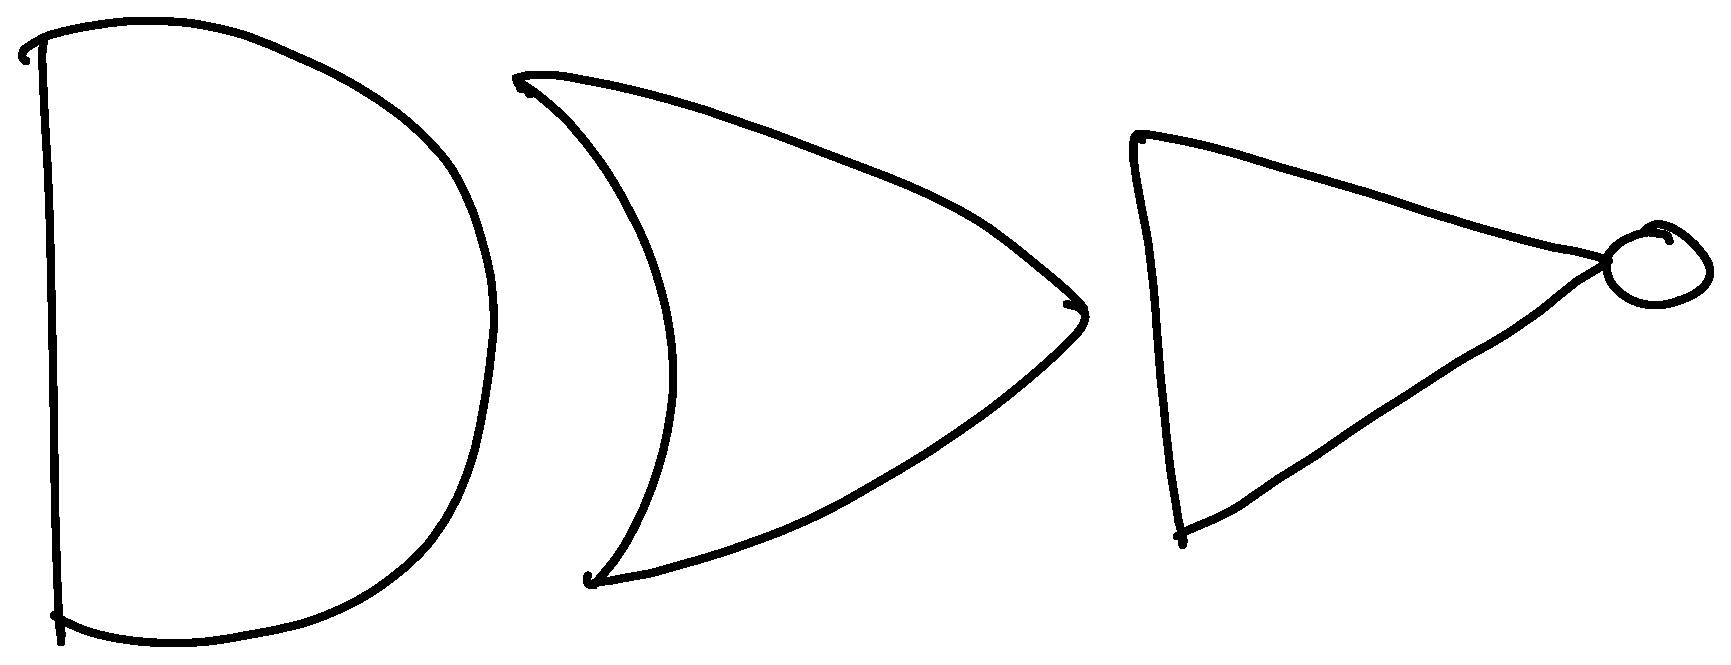
\includegraphics[width=1.0\hsize]{gates}
%\else 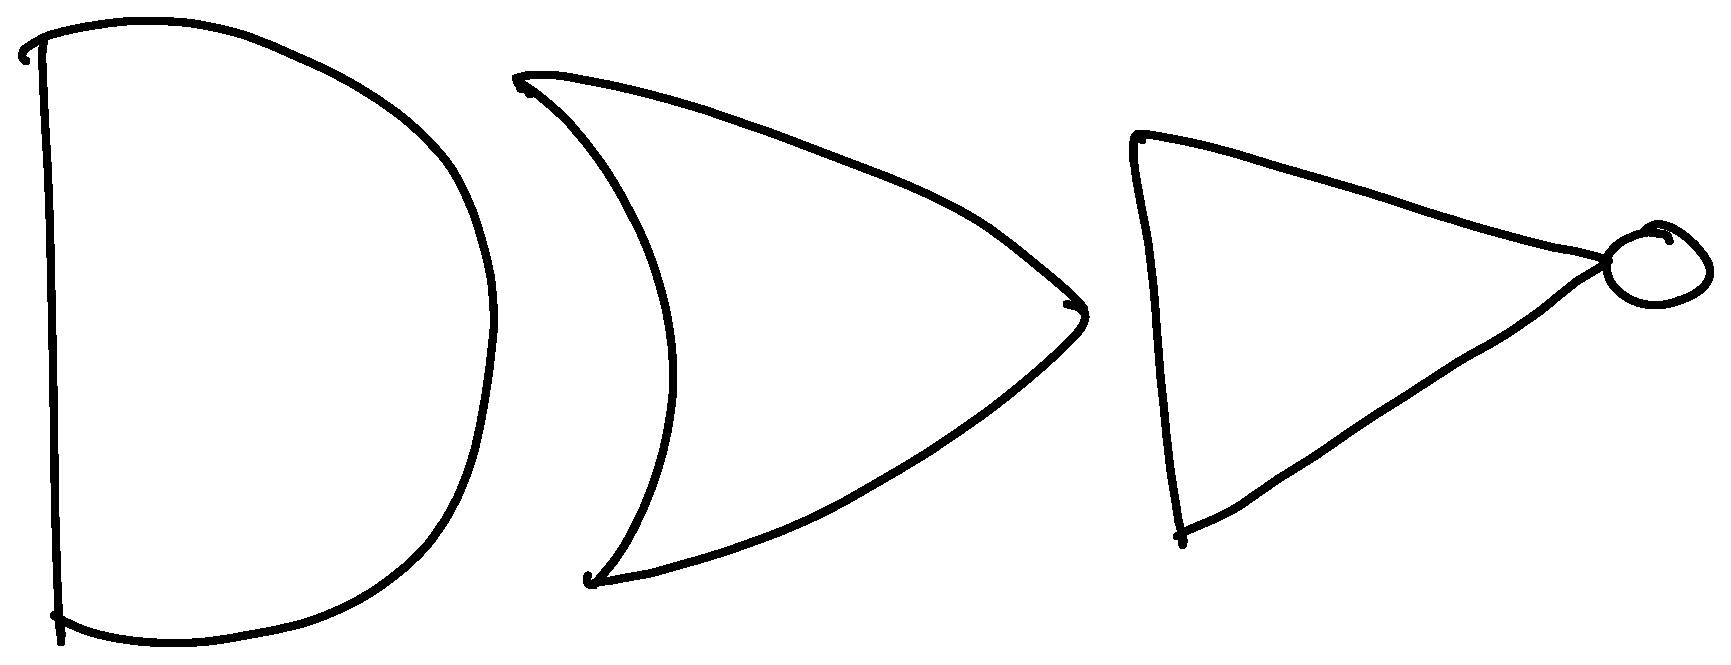
\includegraphics[width=1.0\hsize]{gates.eps} \fi
%\caption{The digital logic gate symbols used in this study. From the left: AND, OR, NOT.}
%\label{gatesFig}
%\end{figure}


\subsection{Data Collection}
We collected digital circuit diagram sketch data from 24 subjects, all college students.  We focus on digital logic diagrams because previous work found that students tend to vary their drawing style in this domain~\cite{Alvarado2007Properties}, and recognizing the symbols in this domain is particularly challenging because many symbols look similar. The participants sketched freely on a Tablet PC; the data collection program performed no recognition.

We asked subjects to perform three tasks mentioned above: isolated shape
drawing (ISO), diagram copying (COPY), and diagram synthesis (SYNTH).  In the
ISO task we asked participants to draw ten isolated instances of each single gate: AND, OR, and NOT, the most common gates in digital circuit design.  In the
COPY task participants were asked to copy two entire circuit diagrams (Figure~\ref{copyFig}).  In the
SYNTH task participants were shown the following logical equations (one at a time)
\[
Y1 = (\overline{(AB+C)}\oplus\overline{AC})+B+C \\
\]
\[
Y2 = (\overline{A}+BC)(A\overline{B}+AC+B)
\]
and
told to create a circuit that satisfies each equation.  This task simulates a
real-world activity, as it is analogous to homework problems students typically
complete for a digital circuit design class.  For the copied and synthesized diagrams, 
we use only the AND, OR and NOT gates because there were not enough of the other gates 
for comparison.  Figure~\ref{synthFig} shows an example of one subject's sketch for 
the first equation above.

\begin{figure}
\mbox{
\ifpdf 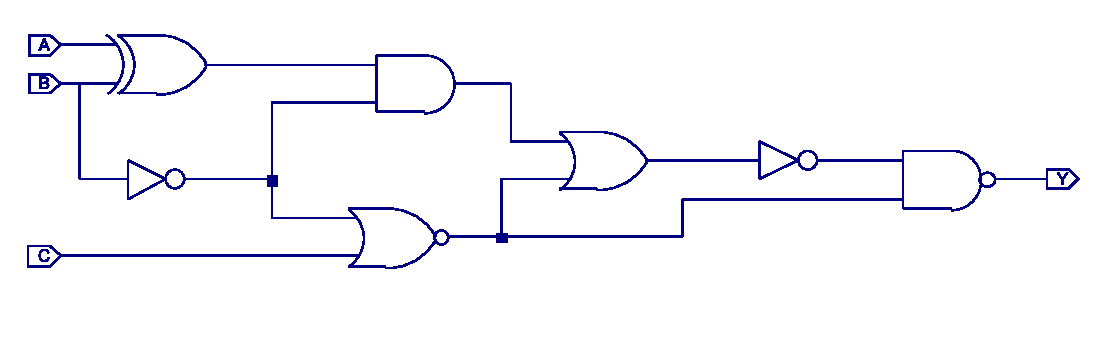
\includegraphics[width=1.0\hsize]{circuit_1}
\else 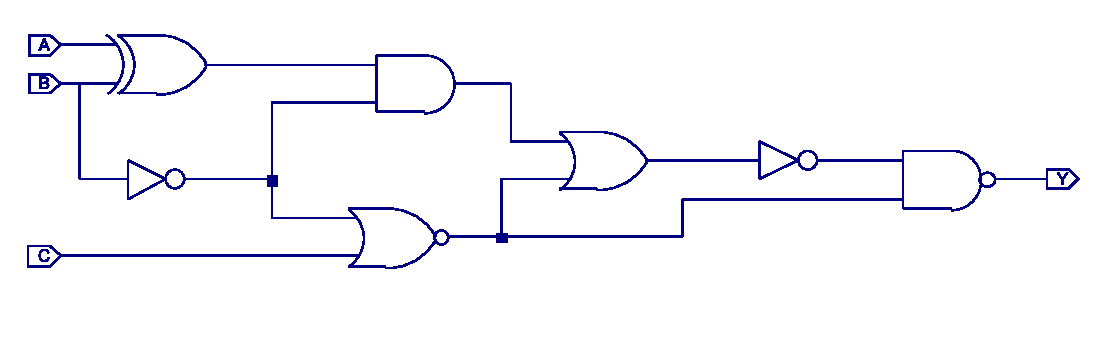
\includegraphics[width=1.0\hsize]{circuit_1.eps} \fi}
\mbox{
\ifpdf 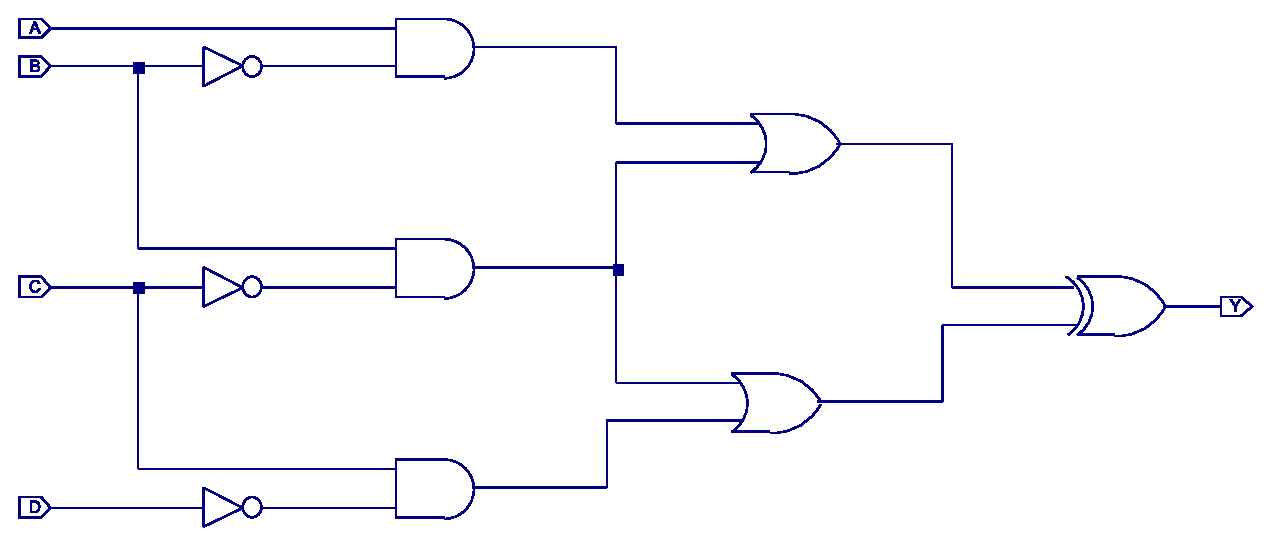
\includegraphics[width=1.0\hsize]{circuit_2}
\else 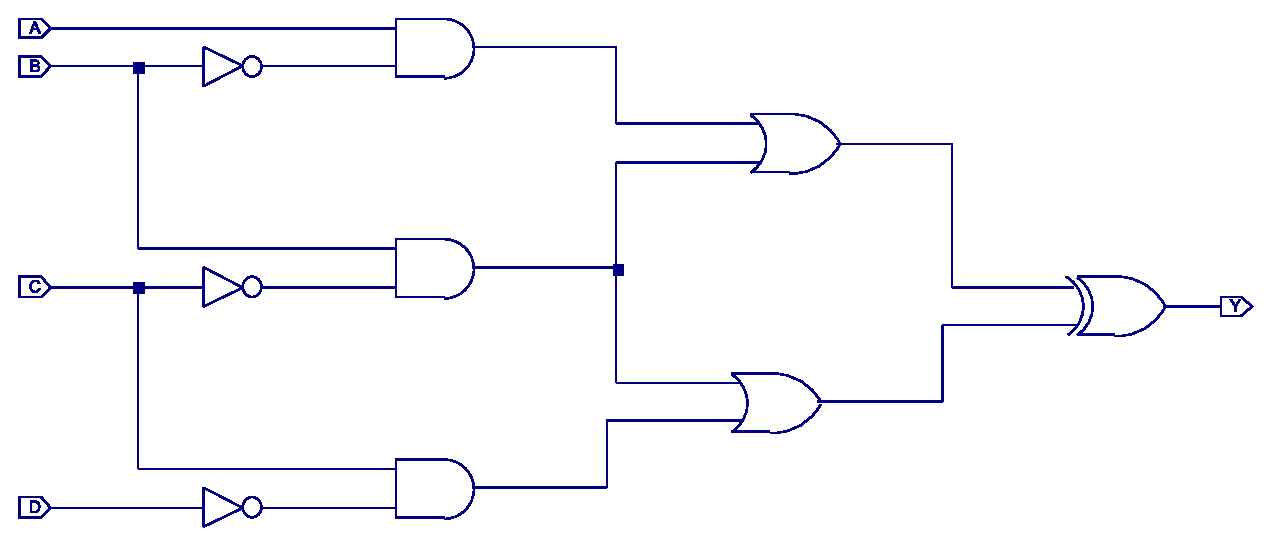
\includegraphics[width=1.0\hsize]{circuit_2.eps} \fi}
\caption{The circuits participants copied in our study}
\label{copyFig}
\end{figure}

\begin{figure}
\ifpdf 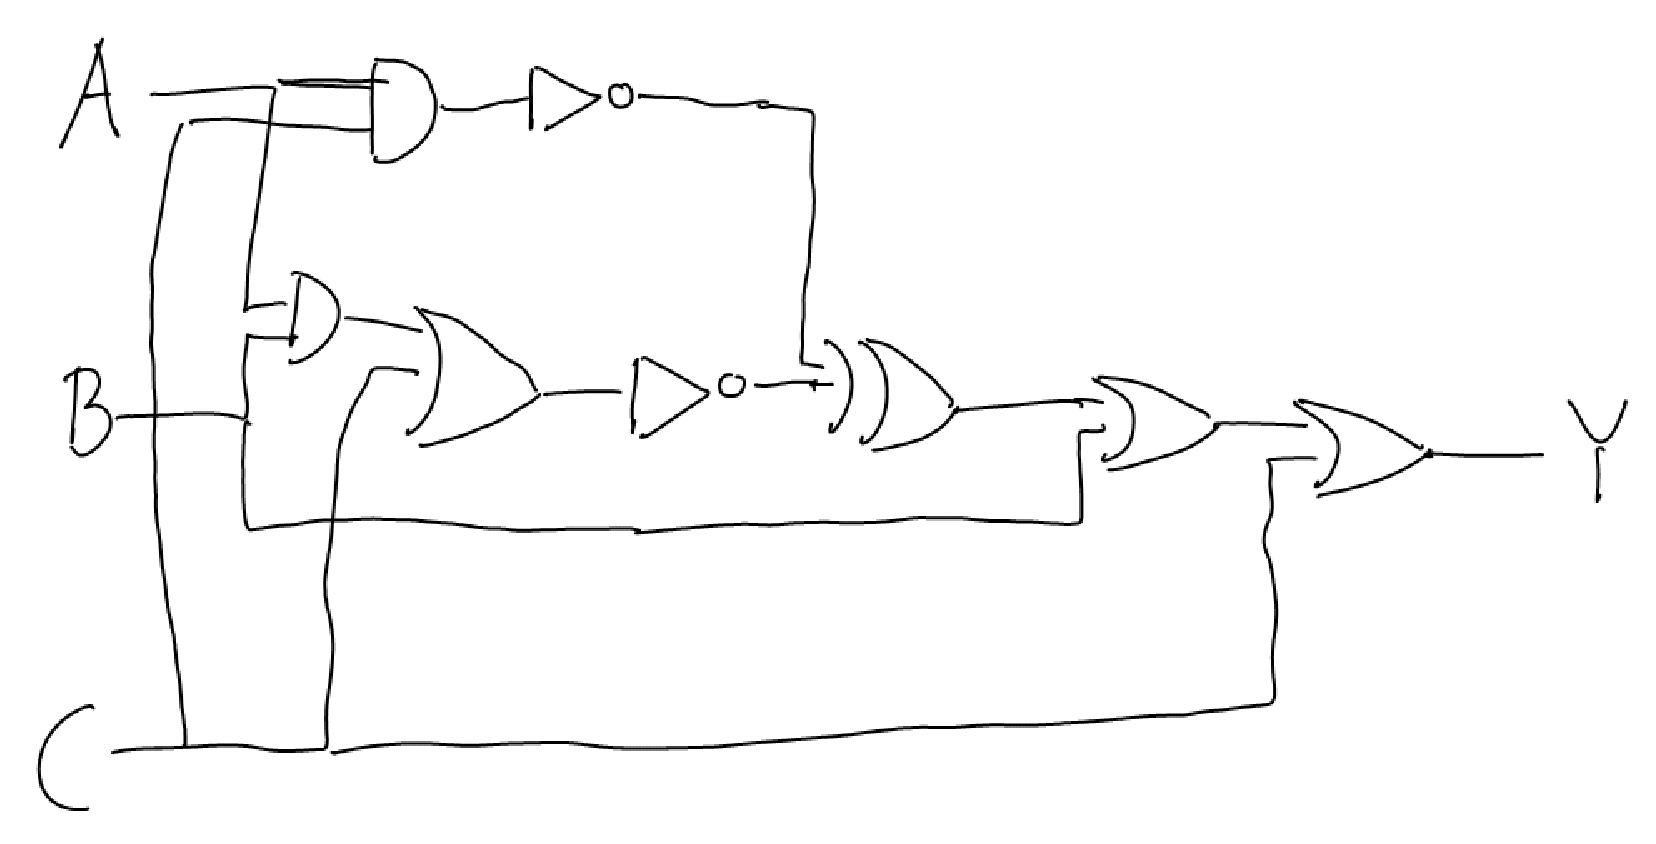
\includegraphics[width=1.0\hsize]{eqDrawing}
\else 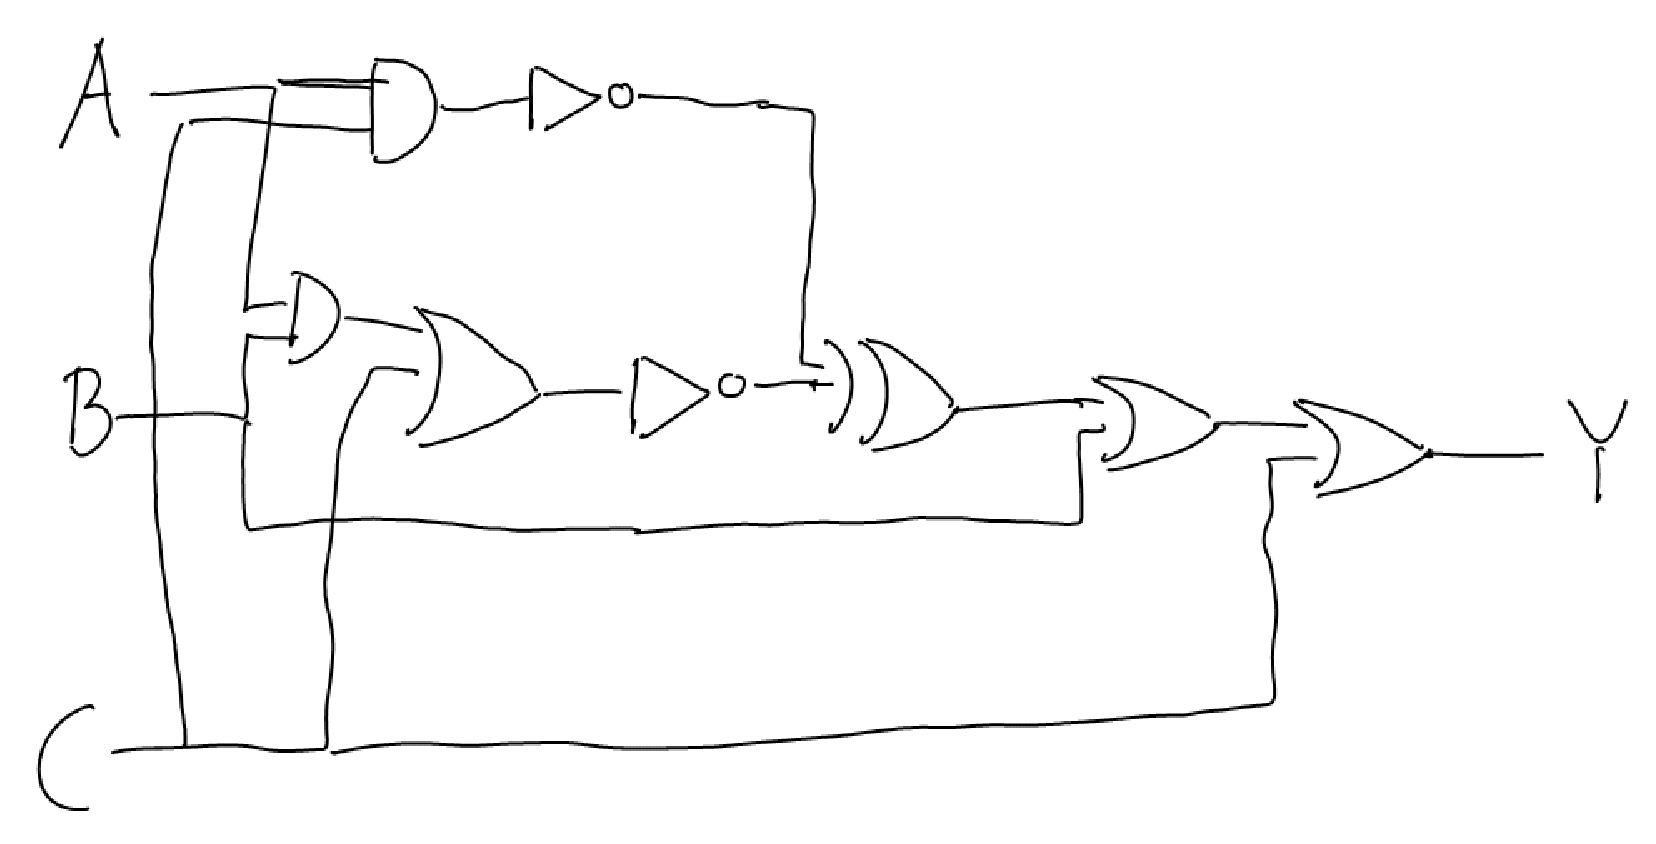
\includegraphics[width=1.0\hsize]{eqDrawing.eps} \fi
\caption{One subject's sketch for the first synthesis equation}
\label{synthFig}
\end{figure}

\subsection{Recognizers}
In our tests we use three distinct recognizers: two modified gesture recognizers\cite{rubine,dollar} and one standard 
image-based symbol recognizer~\cite{Kara2005ImageBased}.  
We chose to include the modified gesture recognizers because we wanted 
to test how sensitive simple gesture recognition techniques are to drawing style.  

The Rubine classifier~\cite{rubine} is a standard and widely-used gesture classifier that works by
extracting features from a single-stroke gesture and then training a linear classifier.  
We used a simple approach to adapt the Rubine classifier to multi-stroke symbols: we simply paste the
strokes together in temporal order.  We then use the same features and the same classification algorithm as
in the original paper.  We expect that this adaptation will be highly sensitive to stroke 
order, so the modified Rubine classifier is the least robust of our three recognizers.

We used a slightly more complex method to adapt our second gesture-based recognizer, the \$1 recognizer,
to handle multi-stroke symbols.
The original single-stroke \$1 recognizer matches a stroke to a template in four stages.   
First, it resamples the points in the 
stroke to be classified so that the stroke and the template contain the same number of points.  Second, it performs 
a crude rotation on the stroke, matching the starting drawing angles between the template and the stroke.  Third, it centers and scales the stroke to match the centroid and scale of the template.  Finally, it refines its rotation to find the angle that results in the smallest path distance between the stroke and the template. 

% The \$1 gesture recognizer required some slightly more complicated
%modifications in order to adapt it to our multiple stroke domain. We will explain how each of the separate steps (resampling, centering and rescaling, rotation search, and distance calculation) were modified.

Our first modification was to the resampling step.  Rather than resampling each stroke to contain the same number of points, we resample each \textit{shape} to contain the same number of points as the template, regardless of how many strokes it contains (we use 48 points in our templates).   We achieve this goal by resampling each stroke to a variable number of points based on the ratio of the stroke's length to the total length of the strokes in the shape so that the total number of points from all the strokes total 48. 

The initial rotation, centering, and rescaling steps remain largely unchanged. Instead of centering on the centroid of one stroke, we use the centroid of the whole symbol. Similarly, we resize the whole symbol to a  $64\times 64$ pixel bounding-box.

%This matching is constrained such that each point in one symbol must match a different point in the other 
%symbol; this way all points are included in the distance calculation. 

In the final step, the rotation search remains the same, but the distance function used to guide the search is heavily modified.  We maintain the one-to-one match between points in the template and points in the symbol to classify, but we can no longer match them based on the order in which they were drawn because we would like our algorithm to be robust to drawing order variation.   We instead compute a matching of points between the two symbols that attempts to minimize the distance between the two symbols. Calculating the actual best match would be prohibitively time-consuming, so we approximate a solution using simulated annealing. We begin the search using the simple greedy solution of matching each point to the nearest available point. We search nearby solutions by picking two points and swapping their matches.

More flexible methods of point-matching, such as Dynamic Time Warping (DTW), have been applied to gesture recognition~\cite{dollar,shark2}. The main difference between these flexible methods and our method is that flexible methods allow multiple points in one shape to be matched to a single point in the other shape. As noted in~\cite{shark2}, a flexible matching of points introduces additional ambiguity between similar templates and degrades the quality of the recognizer.


%In our case, DTW was not an option, because we wanted to relax any assumptions about the ordering of the strokes. Hence any approach dependent on time data would not work. More generally, however, a

We also used the Image-Based Trainable Symbol Recognizer~\cite{Kara2005ImageBased}.  Because this algorithm was originally designed to recognize multiple-stroke shapes, it provides a good contrast to the \$1 and Rubine classifiers. The image-based recognizer is based on template matching, similar to the \$1 recognizer, so it is very easy to add user-specific training examples. Hence, it is especially well suited to both aspects of our testing.

\subsection{Comparison of Recognizers}
Since we completed this work, the authors of the original \$1 recognizer have released (but not yet published) a version suitable for multi-stroke recognition (called the \$N recognizer)\footnote{http://depts.washington.edu/aimgroup/proj/dollar/ndollar.html}.  Their approach is similar to our own, with two differences.  First,  instead of using simulated annealing to match points in the test symbol to points in the template, they order the strokes and then use the same temporal matching techniques as above.  To guard against drawing style variation, they search over the stroke order permutations.   It is not yet clear which approach is superior (if either).  A second important difference between their method and ours is that when they link strokes together, they also consider the ink that was drawn ``in the air'' from the end of one stroke to the beginning of the next.   These virtual points then take away from the total number of points sampled from the actual ink drawn (because the total number of points remains fixed), giving their approach lower resolution and higher sensitivity to variation in shape.

Our modified \$1 recognizer is actually quite similar to the image-based recognizer. Both recognizers preprocess shapes by rescaling and centering them, but where \$1 resamples points, the image-based recognizer rasterizes points into a bitmap image. The next step for both is a rotation search. However, because the image-based recognizer performs its rotation search in polar coordinates, it must also perform a separate distance calculation in screen coordinates once the ideal angle has been located. To perform classification, both recognizers compare the unknown symbol to each of the training examples.

Although the general process is very similar for both recognizers, the small differences have implications for how each performs. The image-based recognizer is extremely robust to noise like overstroking, touch-up strokes, or differing numbers of strokes in the unknown symbol and the template. The modifications we made to the \$1 recognizer attempt to address touch-up strokes or differing numbers of strokes in each shape. However, the resampling process includes the endpoints of all strokes, so with more strokes, the points will be poorly distributed, leading to an increased distance between the unknown shape and template.

The advantage that our modified \$1 has over the image-based recognizer is its simplicity. We tried to stay as much in the spirit of the original \$1 recognizer as possible. The simulated annealing step requires only a small amount of extra code, but adds a large amount of complexity. However, this complexity is still much simpler than the image-based recognizer, especially the rotation search in polar coordinates, and the fact that our recognizer requires only one distance metric rather than the four the image-based recognizer requires.

\section{Experiments and Results}
Our goal with these experiments was threefold.  First, we wanted to examine how task affects recognition accuracy.  Second, we wanted to know how much impact user-specific training data has on recognition accuracy.  Finally, we wanted to compare the modified versions of the simple gesture recognition algorithms with a vision-based recognition algorithm for shapes drawn in the synthesis task (i.e. a task that gesture recognition was not designed to support).

\subsection{The Effect of Task}
\begin{table}
\begin{tabular}{|l||c|c|c|}
\hline
Activity & Rubine & Dollar & Image \\
(train-test) &  & & \\
\hline
Synth-Synth & 21 & 93 & 90\\
Copy-Synth & 39 & 88 & 84\\
Iso-Synth & 53 & 88 & 87\\
Synth-Copy & 39 & 89 & 90\\
Copy-Copy & 54 & 91 & 96\\
Iso-Copy & 48 & 90 & 93\\
Synth-Iso & 32 & 88 & 88\\
Copy-Iso & 43 & 90 & 90\\
Iso-Iso & 53 & 95 & 94\\
\hline
\end{tabular}
\caption{Recognition results for all three recognizers, in percent.}
\label{tab:allResults}
\end{table}

\begin{figure}
\ifpdf 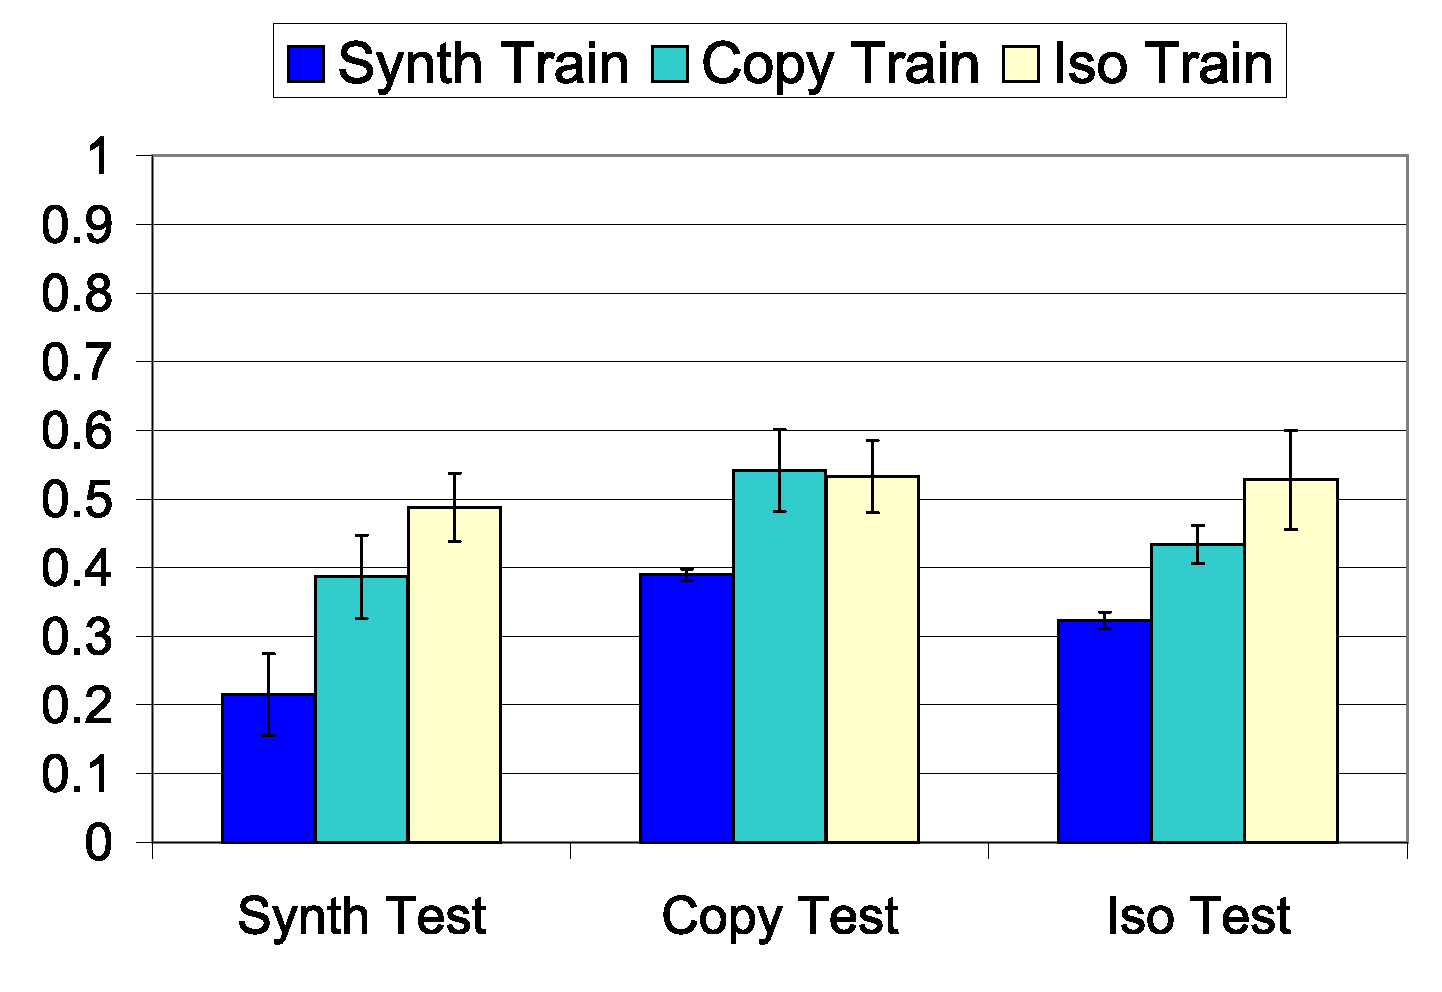
\includegraphics[width=1.0\hsize]{rubine_summary}
\else 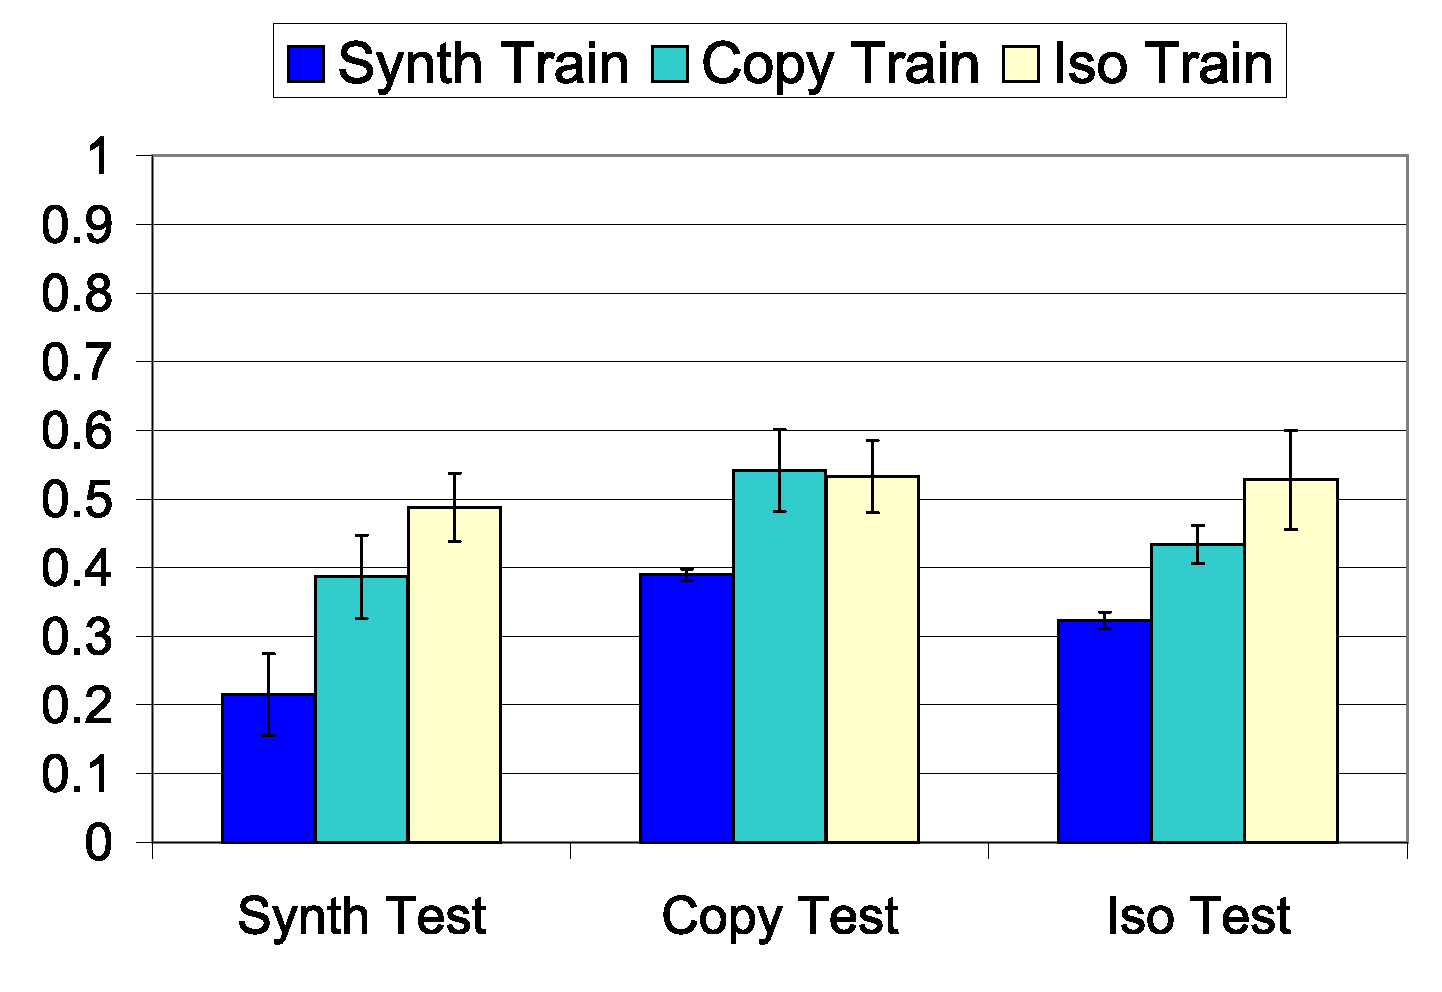
\includegraphics[width=1.0\hsize]{rubine_summary.eps} \fi
\caption{Recognition results for the Rubine recognizer. Error bars show one standard deviation.}
\label{rubineGraph}
\end{figure}

To examine the first question, we separated the data into three categories based on task (ISO, COPY, SYNTH).  We set aside 
data from 80\% of the users (randomly selected) for training and used the data from the remaining 20\% of the users data for testing.  Note that training and testing our recognizers on different user sets simulates the experience of a ``factory trained'' recognizer that cannot be customized to a particular user, which is the normal situation for most sketch recognition systems.  We trained three separate versions of each recognizer on the training data, separated by task.  That is, we trained one Rubine classifier on the ISO training set, a separate Rubine classifier on the COPY set, etc.  The \$1 and image-based recognizers are nearest neighbor classifiers, hence their running time is dependent on the number of training examples.  To achieve reasonable performance, we randomly selected a small subset of the training set to use as templates in these recognizers.  

\begin{figure}
\ifpdf \includegraphics[width=1.0\hsize]{dollar_global_summary}
\else \includegraphics[width=1.0\hsize]{dollar_global_summary.eps} \fi
\caption{Recognition results for the \$1 recognizer.  Error bars show one standard deviation.}
\label{dollarGraph}
\end{figure}

After training, we tested each recognizers on the remaining 20\% in every category (i.e. three test runs for each recognizer).  For example, we ran the ISO Rubine recognizer separately on the test data from the ISO, COPY and SYNTH tasks, for a total of three test runs with this recognizer.  This process resulted in 9 distinct training-testing combinations (iso-iso, iso-copy, iso-synth, copy-iso, etc.).

Table~\ref{tab:allResults} presents the average classification accuracy for all combinations over 25 trials in which we randomly selected a new 80/20 user split for training/testing.  Figures~\ref{rubineGraph},~\ref{dollarGraph}, and~\ref{visionGraph} show these same results graphically, including their standard deviations. For the two recognizers that perform at a reasonable level of accuracy (\$1 and image), task used for training has little if any effect of recognition accuracy (none of these differences are statistically significant using repeated measures ANOVA).  In particular, training on SYNTH data does not appear to improve the accuracy, even when recognizing SYNTH data.  

\begin{figure}
\ifpdf \includegraphics[width=1.0\hsize]{image_global_summary}
\else 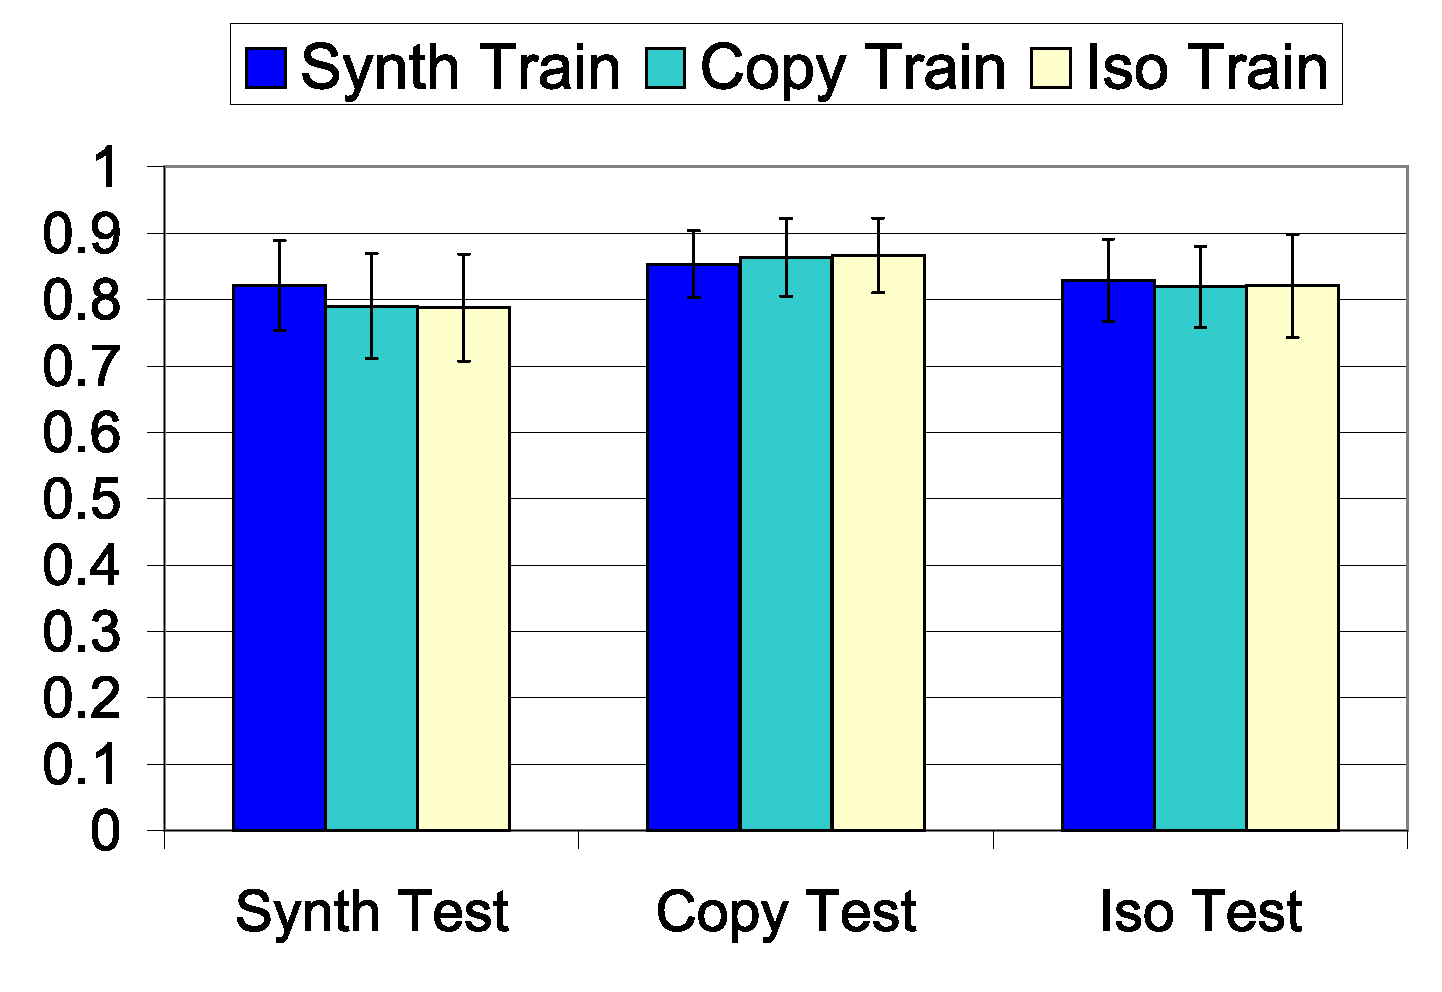
\includegraphics[width=1.0\hsize]{image_global_summary.eps} \fi
\caption{Recognition results for the image-based recognizer. Error bars show one standard deviation.}
\label{visionGraph}
\end{figure}

\subsection{The Effect of User-Specific Data}

To examine the second question, we measured recognition performance as we increased the amount of user-specific training data used to train the recognizer.  

In our first user-data experiment, our goal was to measure the impact of easily collected user-specific data on recognition accuracy in real-world tasks (i.e. the SYNTH task).  In other words, we imagine that the user has acquired a factory-trained recognition system (such as the system produced with the training above), and now has the option of training the system by drawing isolated shapes.  We want to know how much (if at all) this user-specific data will improve classification accuracy.  We focus on only the \$1 and image-based recognizers because of the Rubine classifier's poor performance in the first tests.  

We again split the users into a training set and a testing set as above; however, this time we uses only the SYNTH data for testing and only the ISO data for training.  Again, this choice simulates the situation where the base recognizer was trained in the factory using ISO data from other users, and then trained by the user's individually-drawn symbols.  Note that we use ISO data for the ``factory trained'' recognizer for consistency, but we showed above that any of the datasets produce an equally robust recognizer.

\begin{figure}
\ifpdf \includegraphics[width=1.0\hsize]{user_summary}
\else 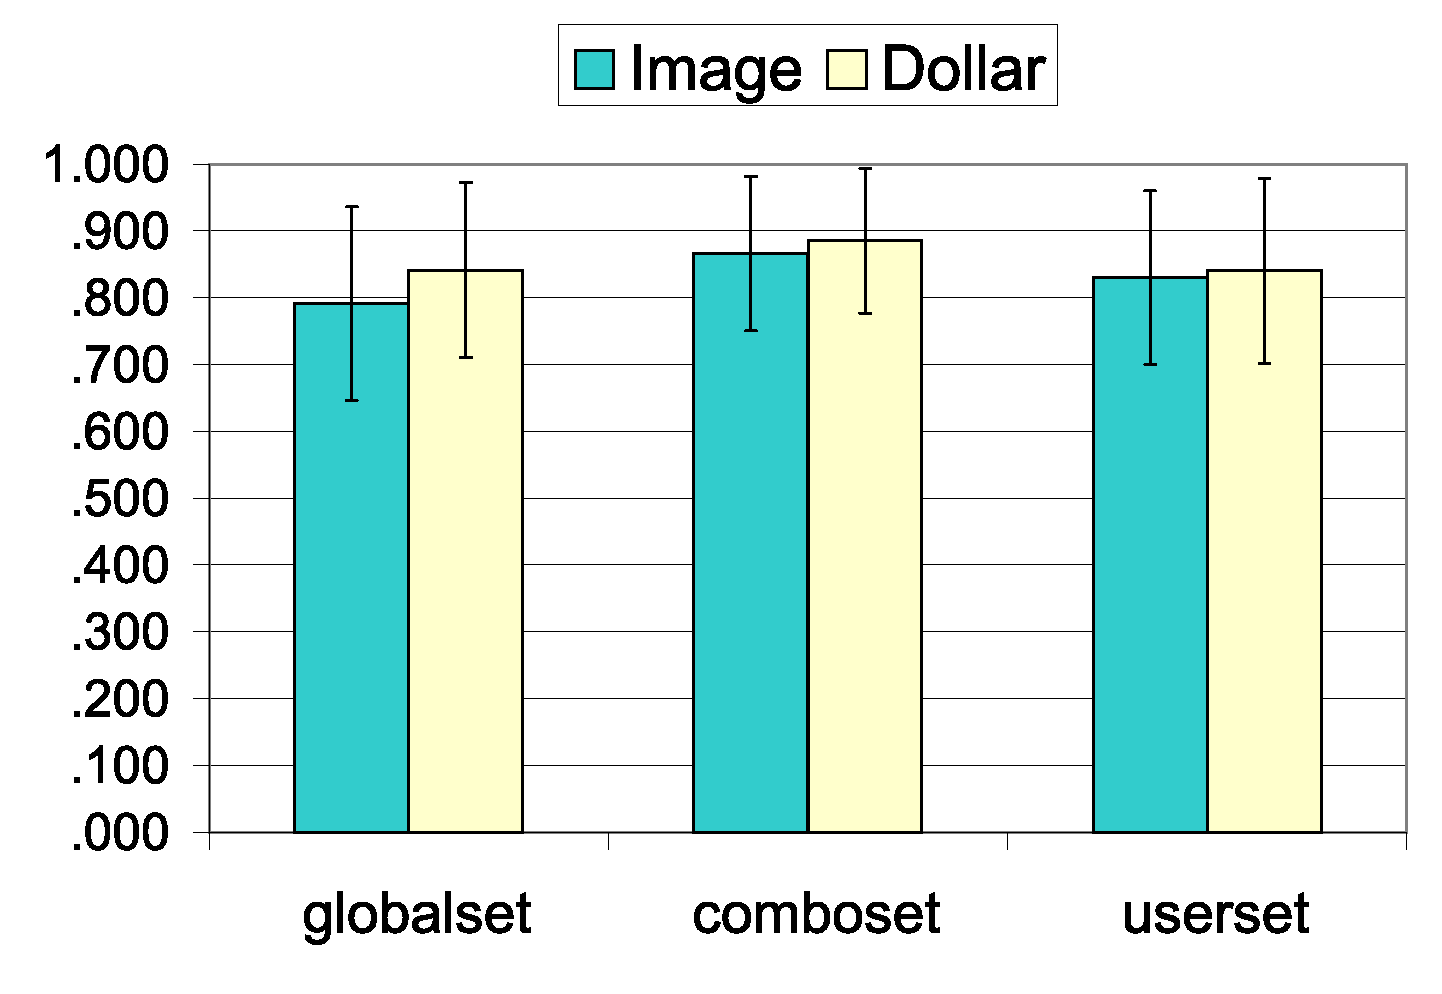
\includegraphics[width=1.0\hsize]{user_summary.eps} \fi
\caption{Recognition results for the \$1 and image-based recognizers with different training sets. Error bars show one standard deviation.}
\label{usersGraph}
\end{figure}

We then generated three of each recognizer (\$1 and image-based) for each user by training the recognizers on training sets containing different amounts of user-specific data.  All of our trials use a constant 5 training examples.  The first training set, called the GlobalSet, contains 5 training examples randomly selected from the 80\% of users in the training set.  (Recall that we use only ISO data for training.)  Because the GlobalSet does not contain user-specific training examples, we used the same GlobalSet for each testing user.  Next, we created a ComboSet recognizer for each user in the testing set by randomly selecting 2 of the GlobalSet training examples and replacing them with 2 randomly selected examples from the testing user's data. We removed the same 2 GlobalSet examples for each user, so the ComboSets differed per-user only in the 2 user-specific examples.  Finally, we created a UserSet recognizer for each user composed solely of 5 examples from the user in question. Hence, the UserSet recognizers are unique to the users they were created for.

\begin{table}
\begin{tabular}{|c|l|l|}
\hline
Recognizer & Comparison & P - Bonferroni \\
\hline
 & GlobalSet and ComboSet & \textbf{0.001} \\
\$1 & UserSet and ComboSet & \textbf{0.001} \\
 & GlobalSet and UserSet & 1.000 \\
\hline
 & GlobalSet and ComboSet & \textbf{<0.001} \\
image-based & UserSet and ComboSet & 0.074 \\
 & GlobalSet and UserSet & 0.144 \\
 \hline
\end{tabular}
\caption{Repeated measures ANOVA Post Hoc results comparing user-independent and user-dependent recognizers}
\label{anovaTable}
\end{table}

Figure~\ref{usersGraph} shows the results of this experiment, averaged over all runs and all users.  While the ComboSet appears to produce the best recognizer, the graph obscures the variations for each individual user and each individual trial.  When we focus on the individual trials, we find that differences in the training sets lead to significantly different classification accuracies.  Table~\ref{anovaTable} gives the results of our repeated measures ANOVA.  We used the Bonferroni correction to reduce the chance of type 1 error. 

\begin{figure}
\ifpdf \includegraphics[width=1.0\hsize]{dollar_image_combo}
\else 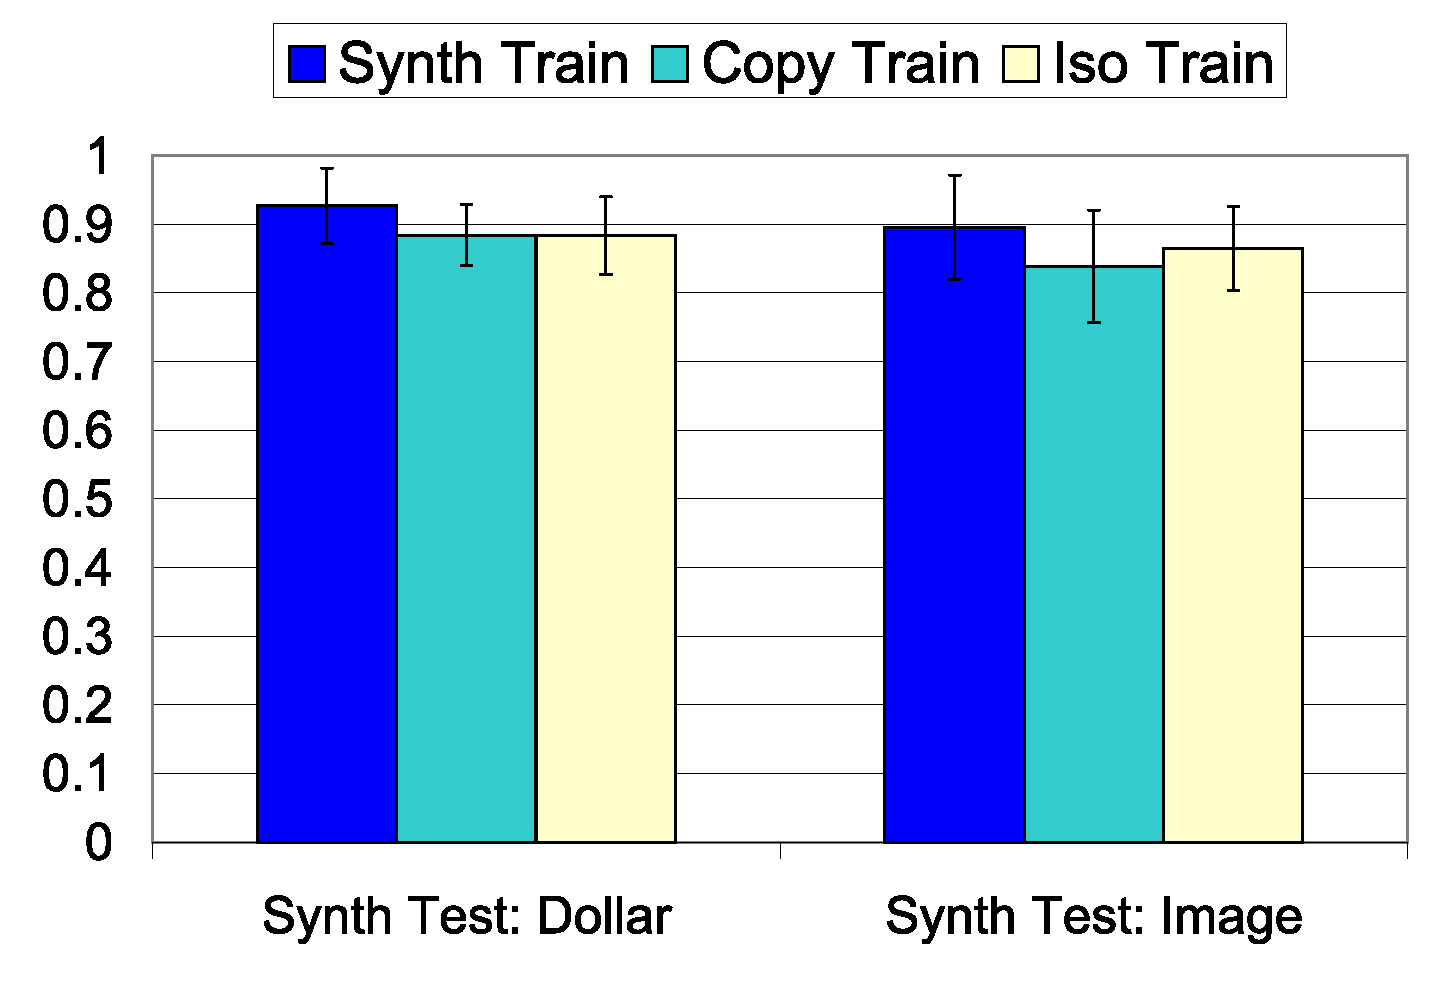
\includegraphics[width=1.0\hsize]{dollar_image_combo.eps} \fi
\caption{Recognition results from the \$1 and image recognizers, trained on different tasks using some user-specific data.  Error bars show one standard deviation.}
\label{comboGraph}
\end{figure}

With the knowledge that user-specific ISO data does in fact improve recognition accuracy, we then investigated 
whether user-specific SYNTH data might improve recognition accuracy even more for SYNTH recognition.  For this experiment, we again focused only on the SYNTH task for recognition and we focus on training sets that have a mix of user-specific and generic data, as in the ComboSet above.  We generated three different training sets for each user, one for each task.  All three sets contain three generic shape examples and two user-specific examples, as above in the ComboSet.  The sets differ only in which tasks subjects performed when generating this data: in the first set we use only SYNTH data, in the second we use only COPY data, and in the third we use only ISO data.  Note that the results from the ISO-trained data will be identical to the results from the ComboSet in Figure~\ref{usersGraph}.

Figure~\ref{comboGraph} shows the results of this experiment for both recognizers.  This graph shows that training on the SYNTH data does in fact give a slight boost to recognition performance over at least one recognizer.  For the \$1 recognizer, it significantly improves performance over the ISO or the COPY data.  For the image-based recognizer, training on the SYNTH data significantly improves performance over training on the COPY data (but not the ISO data).  Table~\ref{anovaTable2} gives the results of our repeated measures ANOVA Post Hoc tests using Bonferroni correction.



\begin{table}
\begin{tabular}{|c|l|l|}
\hline
Recognizer & Comparison & P - Bonferroni \\
\hline
 & Iso train and Copy train & 1.000 \\
\$1 & Iso train and Synth train & \textbf{0.011} \\
 & Copy train and Synth train & \textbf{0.019} \\
\hline
 & Iso train and Copy train  & 0.573 \\
image-based & Iso train and Synth train & 0.369 \\
 & Copy train and Synth train & \textbf{0.033} \\
 \hline
\end{tabular}
\caption{Repeated measures ANOVA Post Hoc results comparing task for user-dependent recognizers}
\label{anovaTable2}
\end{table}

\subsection{The Effect of the Recognizer}
Finally, in all cases, the \$1 and image-based recognizers performed comparably and with reasonably high accuracy.  Unfortunately, we ran the image-based and \$1 tests over different random samples of data, so we cannot directly compare performance using a repeated-measures test (which would be more sensitive to differences in accuracies), but using aggregate statistics, there is no significant difference between the results given by the two classifiers.  This result illustrates the promise of our new modified \$1 recognizer for non-gesture recognition tasks.
%-------------------------------------------------------------------------

\section{Discussion}
In this section we consider the implications of our findings on the general task of free-sketch recognition.  

First, it seems clear that not all gesture recognizers will generalize easily to non-gesture recognition tasks, as evidenced by the poor results of the Rubine recognizer.   The simple methods we used to generalize the Rubine classifier to multiple-stroke shapes did not produce an effective free-sketch recognizer likely because of because of variations in drawing order and sensitivity of some of the Rubine features to stroke end-points.Because the Rubine accuracy is so low, we focus on the \$1 and image-based results for the rest of our discussion.

The \$1 recognizer performed very well across the board. The accuracies of the modified \$1 even begin to approach the accuracies originally presented by Wobbrock et al\cite{dollar}.  The \$1 recognizer was presented originally as an easy-to-implement, highly accurate recognizer for gesture recognition.  Our modification has produced an easy-to-implement, highly accurate recognizer for symbol recognition in freely-drawn sketches.

Our result that training task does not significantly recognition performance when the recognizer is used for other task is very good news for sketch recognition researchers.  As discussed throughout this paper, isolated shapes are much easier to collect and label than truly freely-drawn sketches.  Researchers can use this type of data to train their shape recognizers and these shape recognizers can be adapted to the individual users by having the users draw a few examples of each shape in isolation.

Our second experiment indicates that it is important to include user-specific training examples whenever possible.  The ComboSet performs significantly better than the GlobalSet for both recognizers.  Additionally, for the \$1 recognizer, the ComboSet also significantly outperformed the UserSet. This result can be explained by variation within individual users' drawing styles. The ComboSet contains a wider breadth of examples (from the GlobalSet contribution) than the UserSet, and is hence able to better accommodate this variation. On the other hand, for the image-based recognizer, we cannot safely say that the ComboSet outperformed the UserSet. This result is likely because the image-based recognizer is more robust than our modified \$1, so there is less benefit from the breadth of the GlobalSet. 

The results of our third test indicate that collecting task-specific user training data can aid recognition accuracy even more.  While this type of data seems difficult to collect (no user will group and label their complete sketches), we might be able to leverage the error correction process to obtain this data.  For example, every time the user corrects a classification error in their freely drawn sketch, the system can record this example and user it to train the recognizer.  

The high performance of the modified \$1 and image-based classifiers
%% Rubine accuracy is also low for same-task classification, so I don't see the
%% connection here...
%combined with the low performance of the modified Rubine classifier 
shows that while drawing \textit{style} may vary between tasks, drawing \textit{shape} remains similar.  We expect that our task-specific results would generalize to any other shape-based recognition algorithm, but not to algorithms that depend on stroke drawing order.

%The low accuracy of the Rubine classifier is also a testament to the importance of user-specific training data. The most likely cause of the Rubine classifier's poor performance is the high variability in the way different users draw the same shape.

%We chose to work with the modified Rubine and \$1 recognizers because we hoped to capture as much information about how shapes were drawn as possible. We also wanted to use the image-based recognizer because it could be used exactly as published. We will use the results from these three classifiers to attempt to generalize our conclusions to other systems.

% I'm not really sure I believe this paragraph because we made so many modifications to the dollar 
% to take care of drawing style variations.
%Because of the gesture-classification roots of the Rubine and \$1 classifiers, our modified versions should be at least somewhat sensitive to changes in drawing style. The high accuracy of the isolated-shapes-trained \$1 recognizer implies that there is little difference between the shapes drawn in each activity. Thus, we believe that our results generalize to other types of classifiers. This hypothesis is validated by the results of the image-based recognizer, which also performed very well in the iso-synth test.

Finally, our results show the importance of using easily retainable recognizers for free-sketch recognition.  The \$1 and image-based recognizers support online learning with very little effort or time required. Furthermore, these recognizers only need a small number of examples for training, requiring little extra work from the user to benefit from increased recognition accuracy. However, there are many recognizers for which it is not feasible to incorporate user-dependence in a user-friendly way. For example, some recognizers might need to rerun the entire training process, requiring a long computation. Other recognizers might need to collect many examples from a user before any effect on recognition would be noticed. As we can see in Figure \ref{usersGraph}, the benefit from user-dependence, while significant, are probably not worth too much hassle to a user.



%-------------------------------------------------------------------------
\section{Conclusion}

We have shown that it is possible to train a highly accurate recognizer using only isolated shapes as training data. This is important because isolated shape data is much easier to collect than naturally drawn shapes. It is also much easier to group and label isolated shapes than complicated diagrams.  We have also shown that whenever possible, user-specific examples should be incorporated into training. For classifiers like the image-based and \$1 recognizers, that support online learning, user-specific examples are an easy way to improve accuracy.

%-------------------------------------------------------------------------

\bibliographystyle{eg-alpha}

\bibliography{gatestudy}

\end{document}
